%Review of existing harmonic excitation.
%	Nonlinear Systems
%		Traditional Metrics (THD, IMD)
%		Minimisation of Nonlinear Distortion
%		Advent of "Nonlinear Niceness"
%	Timbre of nonlinear distortions (Martens and Marui type shit)
%	Uses of Harmonic Excitation
%	Harmonic Generation Methods
%		Static Nonlinearities
%		Bandwidth Extension (high frequency reconstruction)
%		Individual Harmonic Generation (SMC paper)
%		Psychoacoustic Enhancers

\chapter{Harmonic Excitation}
\label{chap:Excitation}

\section{Introduction}
\label{sec:Excitation-Introduction}
	\note{Harmonic excitation is of the chain. Look I wrote a paper about it \citep{enderby2013methods}.}

\section{Nonlinear Systems}
\label{sec:Excitation-NonlinearSystems}
	\note
	{
		THD and IMD are rubbish but served some purpose in the olden days. Some more metrics were made but they 
		were still only concerned with minimising distortion \citep{lee2003auditory, geddes2003auditory, 
		tan2004predicting}. \citet{voishvillo2006assessment} summarises a lot of metrics nicely. Then some bloke 
		decided distortion was cool.
	}

\section{Timbre of Nonlinear Distortion}
\label{sec:Excitation-Timbre}
	\note
	{
		Marui and Martens did some of this \citep{marui2005timbre, marui2005constructing, marui2005predicting}.
	}

\section{Uses of Harmonic Excitation}
\label{sec:Excitation-Uses}
	\note
	{
		Psychoacoustic reproduction of low frequency signals on small loudspeakers as done by 
		\citet{larsen2002reproducing} and \citet{gan2001virtual}.

		Reconstruction of high frequency components after lossy data compression \citep{friedrich2007spectral, 
		nagel2009a, nagel2010a, valin2000bandwidth, dietz2002spectral, larsen2002efficient, sha2010high}.

		Applications in increasing the intelligibility of speech.
	}

\section{Evaluation Methodology}
\label{sec:Excitation-Evaluation}
	\begin{itemize}
		\item Low Complexity.
		\item Predictable, consistent behaviour (homogeneity).
		\item Spectral Characteristics.
		\item Temporal Characteristics.
		\item Preservation of harmonicity (low IMD).
		\item Control over order of harmonics generated.
		\item Naturalness of generated harmonics.
	\end{itemize}

\section{Harmonic Generation Methods}
\label{sec:Excitation-Methods}
	\note{I like to generate harmonics, basically a nonlinear process}

	\subsection{Static Nonlinearities}
	\label{sec:Excitation-Statics}
		Static nonlinearities are simple mappings between input value and output value. A very basic static
		nonlinearity is a symmetric hard clipping system as shown in Equation \ref{eq:SymmetricHardClipping}.

		\begin{equation}
			y(n) = \begin{cases}
				t & \text{if $x(n) > t$} \\
				x(n) & \text{if $|x(n)| \leq t$} \\
				-t & \text{if $x(n) < -t$}
			\end{cases}
			\label{eq:SymmetricHardClipping}
		\end{equation}

		\subsubsection*{Complexity}

		\subsubsection*{Homogeneity}
			\note{DAFx Paper}

			The inhomogeneity of simple clipping systems can be counteracted by introducing gain stages either
			side of the clipping stage. The first gain stage scales the signal so that the clipping stage will
			always clip the same proportion of the signal. The second gain stage scales the signal back to the
			original input amplitude. Analogously the clipping function can be scaled so as to always clip the
			same proportion of the signal, as done by \citet{deman2014adaptive}.

		\subsubsection*{Spectral Characteristics}
		\subsubsection*{Temporal Characteristics}
		\subsubsection*{Preservation of Harmonicity}
		\subsubsection*{Flexibility}
		\subsubsection*{Naturalness}

	\subsection{Rectification}
	\label{sec:Excitation-Rectification}
		\begin{equation}
			y(n) = \begin{cases}
				0 & \text{if $x < 0$} \\
				x(n) & \text{otherwise}
			\end{cases}
			\label{eq:Half-Wave-Rectification}
		\end{equation}

		\begin{equation}
			y(n) = |x(n)|
			\label{eq:Full-Wave-Rectification}
		\end{equation}

		\subsubsection*{Complexity}
		\subsubsection*{Homogeneity}
		\subsubsection*{Spectral Characteristics}
		\subsubsection*{Temporal Characteristics}
		\subsubsection*{Preservation of Harmonicity}
		\subsubsection*{Flexibility}
		\subsubsection*{Naturalness}

	\subsection{Integrator}
	\label{sec:Excitation-Integrator}
		\begin{equation}
			y(n) = \begin{cases}
				0 & \text{if $x(n) > 0$ and $x(n - 1) \leq 0$} \\
				y(n - 1) + c|x(n)| & \text{otherwise}
			\end{cases}
			\label{eq:Integrator}
		\end{equation}

		\subsubsection*{Complexity}
		\subsubsection*{Homogeneity}
		\subsubsection*{Spectral Characteristics}
		\subsubsection*{Temporal Characteristics}
		\subsubsection*{Preservation of Harmonicity}
		\subsubsection*{Flexibility}
		\subsubsection*{Naturalness}

	\subsection{Multiplier}
	\label{sec:Excitation-Multiplier}
		\begin{equation}
			y(n) = x(n)^{h}, \quad h \in \mathbb{N}
			\label{eq:Multiplier}
		\end{equation}

		\subsubsection*{Complexity}
		\subsubsection*{Homogeneity}
		\subsubsection*{Spectral Characteristics}
		\subsubsection*{Temporal Characteristics}
		\subsubsection*{Preservation of Harmonicity}
		\subsubsection*{Flexibility}
		\subsubsection*{Naturalness}

	\subsection{Single Side Band Automodulation}
	\label{sec:Excitation-SSB}
		Single sideband automodulation utilises the concept of single sideband modulation
		\citep{corinthios2009signals}. This allows you to apply amplitude modulation to a signal and only produce
		either the sum or difference sideband.

		A simple way to apply single sideband modulation to a signal is through construction of an analytic signal.
		An analytic signal is a complex valued signal, the real part of which is the original signal and the
		imaginary part its Hilbert transform. The analytic signal is often denoted with a subscript letter
		$a$, such that the analytic representation of the signal $x(n)$ would be denoted $x_{a}(n)$.

		In single sideband automodulation the analytical representation of the input signal is multiplied with
		itself in order to generate harmonics. Equation \ref{eq:SSB} shows the $h^{\text{th}}$ order single side
		band auto modulation of a signal.

		\begin{equation}
			y(n) = \Re \left( x_{a}(n)^{h} \right), \quad h \in \mathbb{N}
			\label{eq:SSB}
		\end{equation}

		\subsubsection*{Complexity}
		\subsubsection*{Homogeneity}
		\subsubsection*{Spectral Characteristics}
		\subsubsection*{Temporal Characteristics}
		\subsubsection*{Preservation of Harmonicity}
		\subsubsection*{Flexibility}
		\subsubsection*{Naturalness}

	\subsection{Instantaneous Amplitude and Phase}
	\label{sec:Excitation-IAP}
		\begin{equation}
			y(n) = |x_{a}(n)| \cos \left( h\arg(x_{a}(n)) \right), \quad h \in \mathbb{N}
			\label{eq:IAP}
		\end{equation}

		\subsubsection*{Complexity}
		\subsubsection*{Homogeneity}
		\subsubsection*{Spectral Characteristics}
		\subsubsection*{Temporal Characteristics}
		\subsubsection*{Preservation of Harmonicity}
		\subsubsection*{Flexibility}
		\subsubsection*{Naturalness}

	\subsection{Spectral Replication}
	\label{sec:Excitation-SpectralReplication}
		The principle behind spectral replication is to reproduce the spectral structure of a signal at higher
		frequencies.

		\begin{figure}[h!]
			\centering
			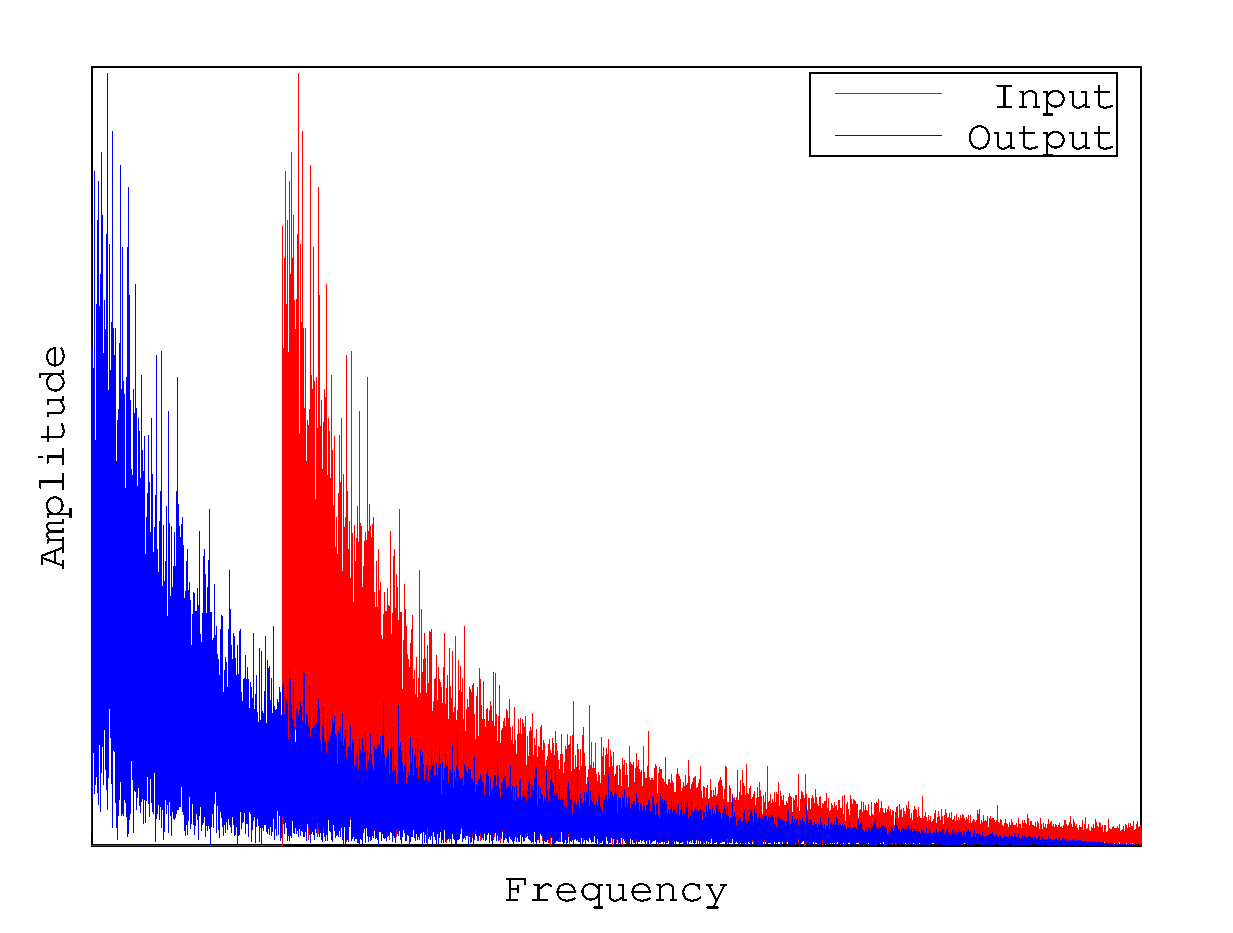
\includegraphics[width=0.6\textwidth]{chapter3/Images/SpectralReplication.eps}
			\caption{The spectral characteristics of spectral replication.}
			\label{fig:SpectralReplication}
		\end{figure}

		This spectral shift is easily implemented through the use of single side band modulation as shown in
		Equation \ref{eq:SpectralReplication}.

		\begin{equation}
			y(n) = \Re \left( x_{a}(n) e^{i\omega  n/ f_{s}} \right)
			\label{eq:SpectralReplication}
		\end{equation}

		Where $\omega$ is the angular frequency the signal should be shifted by and $f_{s}$ is the sampling
		frequency of the signal.

		\subsubsection*{Complexity}
		\subsubsection*{Homogeneity}
		\subsubsection*{Spectral Characteristics}
		\subsubsection*{Temporal Characteristics}
		\subsubsection*{Preservation of Harmonicity}
		\subsubsection*{Flexibility}
		\subsubsection*{Naturalness}

	\subsection{Spectral Folding}
	\label{sec:Excitation-SpectralFolding}
	
		\begin{figure}[h!]
			\centering
			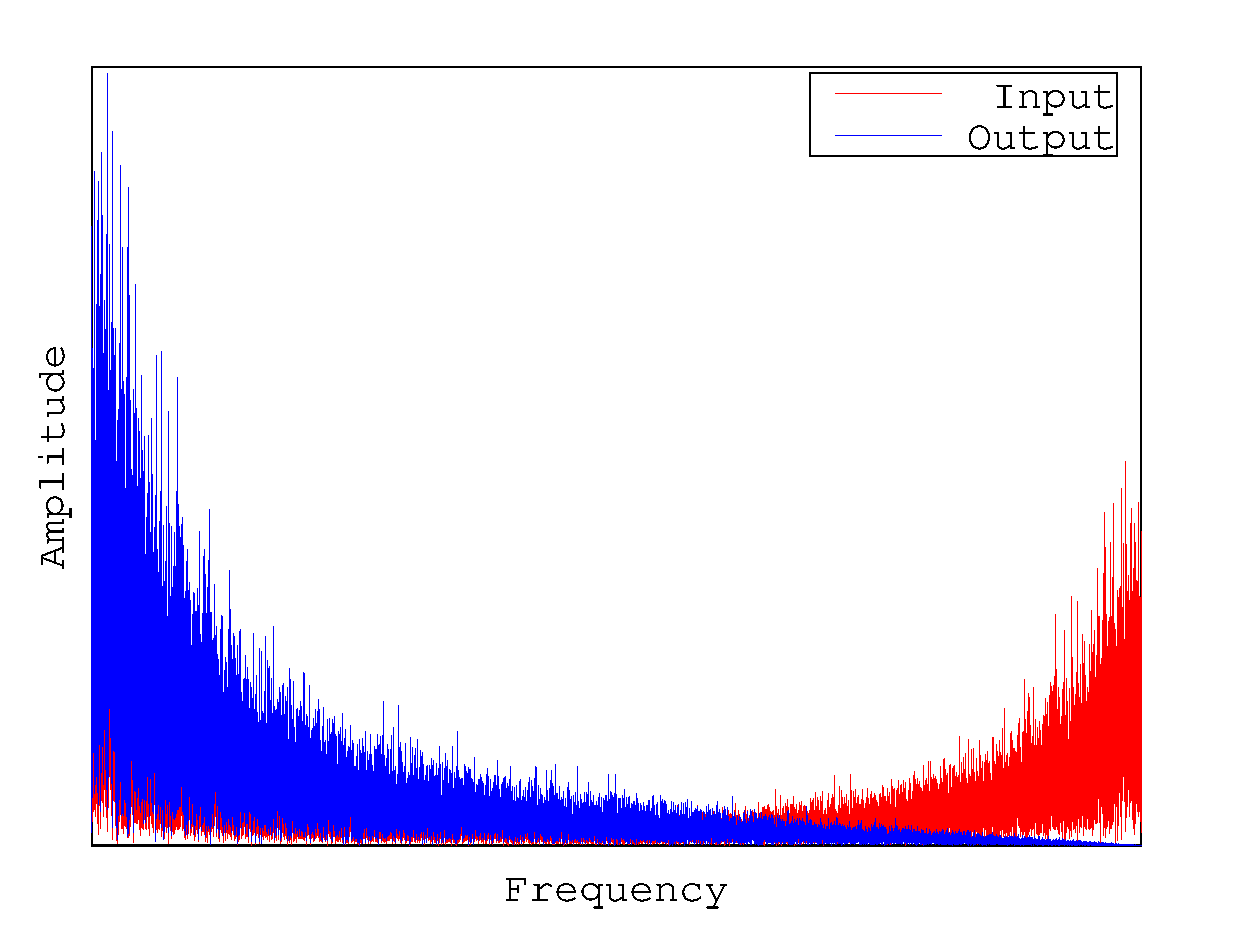
\includegraphics[width=0.6\textwidth]{chapter3/Images/SpectralFolding.eps}
			\caption{The spectral characteristics of spectral folding.}
			\label{fig:SpectralFolding}
		\end{figure}

		\begin{equation}
			y(n) = \begin{cases}
				-x(n) & \text{if $n$ is odd} \\
				x(n) & \text{otherwise}
			\end{cases}
			\label{eq:SpectralFolding}
		\end{equation}

		\subsubsection*{Complexity}
		\subsubsection*{Homogeneity}
		\subsubsection*{Spectral Characteristics}
		\subsubsection*{Temporal Characteristics}
		\subsubsection*{Preservation of Harmonicity}
		\subsubsection*{Flexibility}
		\subsubsection*{Naturalness}

	\subsection{Spectral Stretching}
	\label{sec:Excitation-SpectralStretching}

		\begin{figure}[h!]
			\centering
			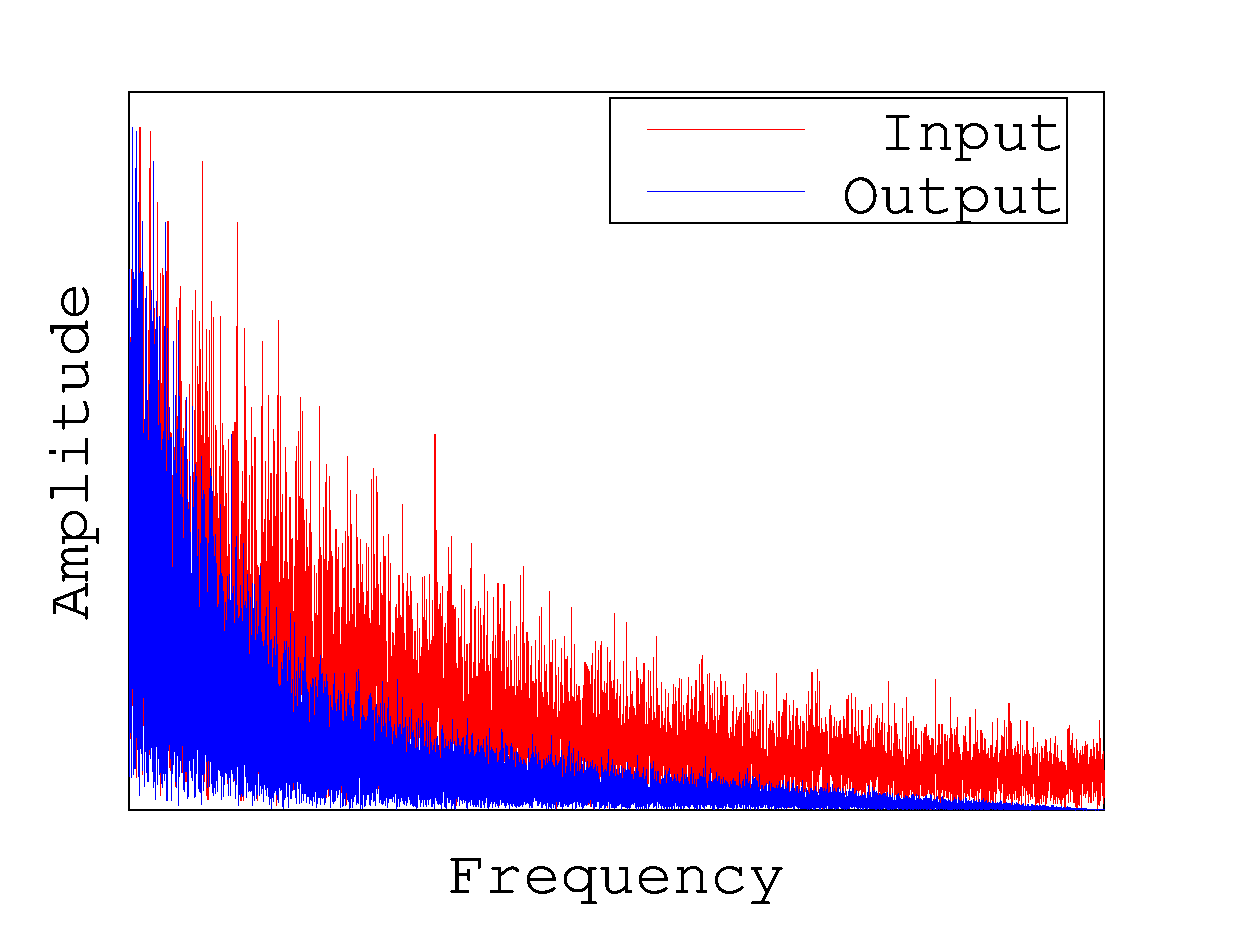
\includegraphics[width=0.6\textwidth]{chapter3/Images/SpectralStretching.eps}
			\caption{The spectral characteristics of spectral stretching.}
			\label{fig:SpectralStretching}
		\end{figure}

		\subsubsection*{Complexity}
		\subsubsection*{Homogeneity}
		\subsubsection*{Spectral Characteristics}
		\subsubsection*{Temporal Characteristics}
		\subsubsection*{Preservation of Harmonicity}
		\subsubsection*{Flexibility}
		\subsubsection*{Naturalness}

	%\subsection{Bandwidth Extension}
	%\label{sec:Excitation-BWE}
	%	\note
	%	{
	%		A nice summary in \citet{larsen2004audio}.

	%		Look at Figure \ref{fig:SpectralFolding} 'aint it fancy.
	%	}

	%	\begin{figure}[h!]
	%		\centering
	%		\subfloat[Spectral Folding]
	%		{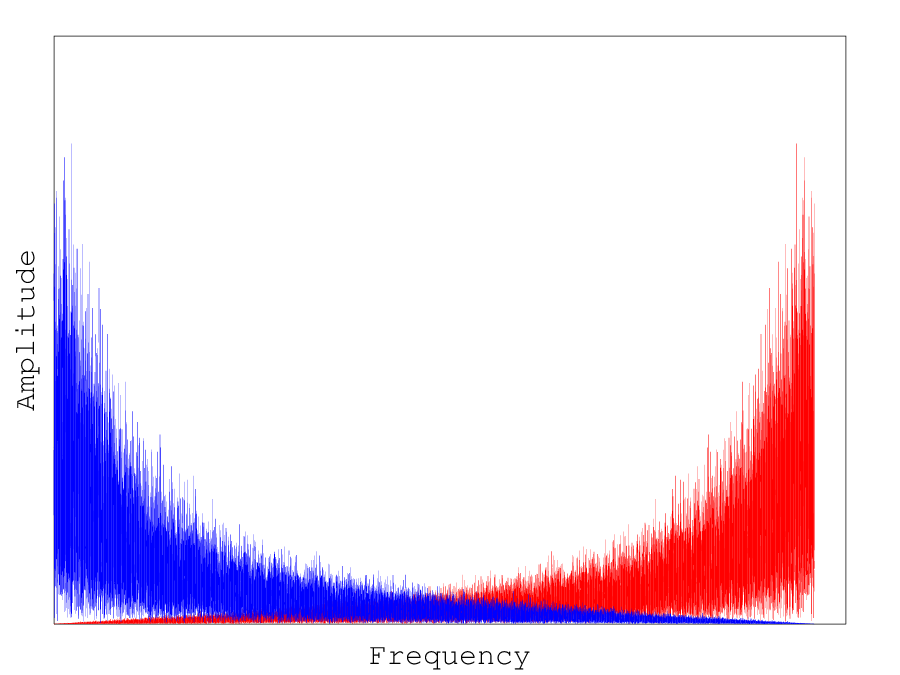
\includegraphics[width=0.4\textwidth]{chapter3/Images/SpectralFolding.png}}
	%		\subfloat[Spectral Replication]
	%		{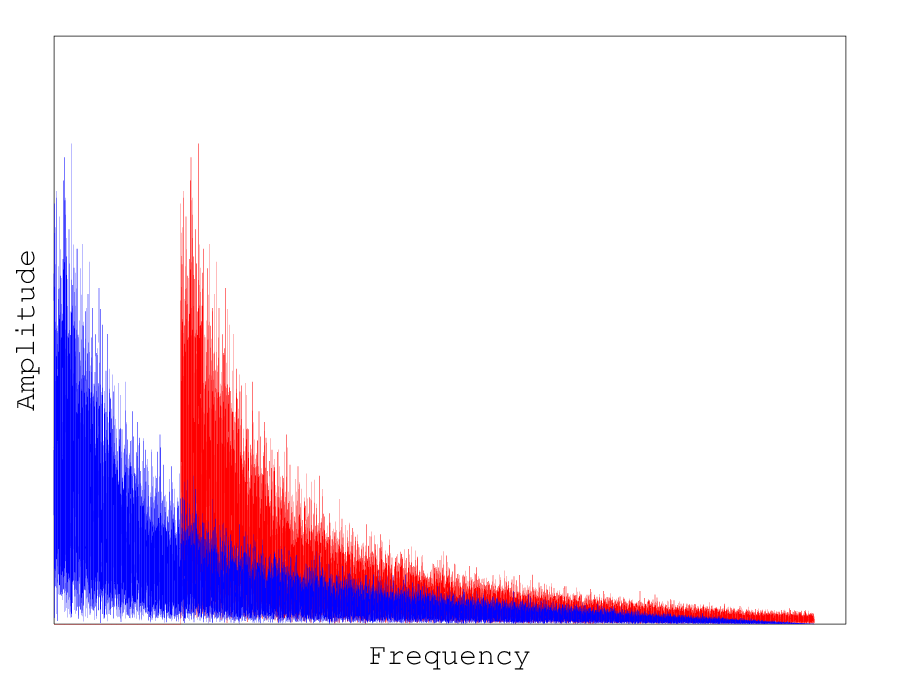
\includegraphics[width=0.4\textwidth]{chapter3/Images/SpectralReplication.png}}
	%		\\
	%		\subfloat[Spectral Stretching]
	%		{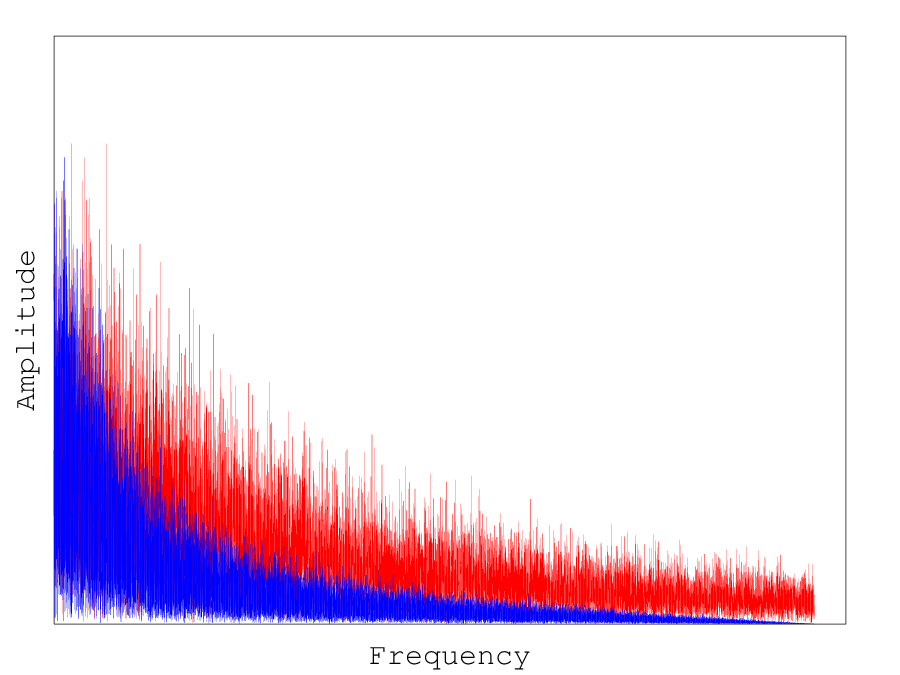
\includegraphics[width=0.4\textwidth]{chapter3/Images/SpectralStretching.png}}
	%		\caption{Spectral characteristics of different band width extension methods. In each graph the blue 
	%		section represents the original spectra and the red section the new spectral content.}
	%		\label{fig:SpectralFolding}
	%	\end{figure}

	\subsection{Individual Harmonic Generation}
	\label{sec:Excitation-Individuals}
		\note{SMC paper}

	\subsection{Psychoacoustic Enhancers}
	\label{sec:Excitation-Enhancers}
		\note
		{
			Probably the most well known perceptual control effects out there. The Aural Exciter has been 
			covered by both \citet{chalupper2000aural} and \citet{shekar2013modeling}.
		}

	\subsection{Fundamental Frequency Tracking}
	\label{sec:Excitation-Fundamental}
		\note
		{
			Several generation methods can be improved through tracking the fundamental frequency of the input 
			signal.

			We can talk all about fundamental / pitch tracking here \citep{cuadra2001efficient, 
			gerhard2003pitch, prukkanon2009vt-amdf, larsen2004audio}.
		}

\begin{landscape}
\section{Methods Comparison}
\label{sec:Excitation-Comparison}

	\begin{tabular}{|c|c|c|c|c|c|c|}
		\hline
		\bf{Method} & \bf{Complexity} & \bf{Homogeneity} & \bf{Spectral Properties} & \bf{Temporal Properties} & \bf{IMD}
		\bf{Flexibility} & \bf{Naturalness} \\
		\hline
		Static Nonlinearity & $\mathcal{O}(n)$ & & & & & \\
		\hline
		Rectifier & $\mathcal{O}(n)$ & & & & & \\
		\hline
		Integrator & $\mathcal{O}(n)$ & & & & & \\
		\hline
		Multiplier & $\mathcal{O}(n)$ & & & & & \\
		\hline
		SSB & $\mathcal{O}(n)$ & & & & & \\
		\hline
		IAP & $\mathcal{O}(n)$ & & & & & \\
		\hline
		Spectral Replicator & $\mathcal{O}(n)$ & & & & & \\
		\hline
		Spectral Mirror & $\mathcal{O}(n)$ & & & & & \\
		\hline
		Spectral Stretch & $\mathcal{O}(n\log{n})$ Assuming FFT used & & & & & \\
		\hline
	\end{tabular}

\end{landscape}
